

\newpage
\section{7-02-2019: DINAMIC DISPATCHING}
Nei linguaggi ad oggetti, lo strumento più potente è la classe. Quando definisco le entità che poi vado a tramutare in classi sto definendo DATI. \newline
Le classi possono contenere dei metodi (funzioni che operano sugli oggetti della classe). \newline
Definire sottoclassi significa definire \textit{sottoinsiemi} nell'ambito dell'ereditarietà. Le nuove operazioni delle sottoclassi vanno inserite sapendo che le sottoclassi ereditano il set di funzioni delle superclassi. 

\noindent \textbf{OVERRIDING} \newline
L'\textit{OVERRIDING} è il punto cruciale di tutta la programmazione ad oggetti. Fare overriding significa sovrascrivere un metodo ereditato dalla super classe per poterne specializzare il suo comportamento. Se non potessi farlo significa che nelle sottoclassi non posso andare a specializzare un metodo. Specializzare un metodo significa cambiare l'implementazione della super classe senza cambiarne la firma. 

\noindent @ serve per creare delle annotazioni nel codice, serve per il compilatore (es: @ override)

\noindent \textit{IL POLIMORFISMO} è uno strumento molto utile perchè ci permette di scrivere codice, funzioni che posso adoperare anche con tipi diversi!

\noindent \textbf{DINAMIC DISPATCHING} \newline
Il \textit{DINAMIC DISPATCHING} serve in fase di runtime a scegliere la versione giusta del metodo da richiamare. Infatti se ho degli over ride nelle mie classi, sarà solo in fase di run time che Java deciderà quale metodo richiamare. Se nella mia classe non esiste il metodo richiamato, il dinamic dispatching va a prendere l'implementazione del metodo dalla superclasse. Nella memoria che contiene le informazioni degli oggetti ci sono tutti i puntatori ai metodi di una classe, in run time viene eseguito il codice del puntatore corretto. (\textit{vedere: virtual table}).
Un \textit{OGGETTO} infatti è costituito da un insieme dei suoi campi e da puntatori ai metodi della classe ed è grazie a questo che il dispatching funziona: il compilatore controlla i tipi e garantisce che nel compiling time tutto questo funzioni. 

\noindent Ogni espressione ha un tipo!

\noindent \textbf{CLASSI E METODI STATICI} \newline
\textbullet\ I metodi statici sono quei metodi di una classe che appartengono alla classe, non alle istanze di una classe. Si possono richiamare senza creare un oggetto. I metodi statici possono quindi accedere solo a dati statici e non alle variabili di istanza della classe, possono solo richiamare altri metodi statici della classe, e sopratutto non possono usare il parametro implicito \textit{this}. \newline
\textbullet\ Le classi statiche in java possono solamente esistere se sono \textit{innestate (nested)}. Esse possono accedere solamente dati statici della classe che le contiene. Una classe statica interna non vede il riferimento this dell'altra classe, essa può accedere solamente ai campi statici della classe che la contiene. 

\noindent Le \textit{COLLECTION} sono delle interfacce della libreria di JAVA e non si possono costruire.\newline
Le \textit{COLLECTION} da sole non sono dei tipi, le \textit{COLLECTION} di un "qualcosa" sono dei tipi.I tipi parametrici vogliono infatti un \textit{argomento} \newline
\begin{center}
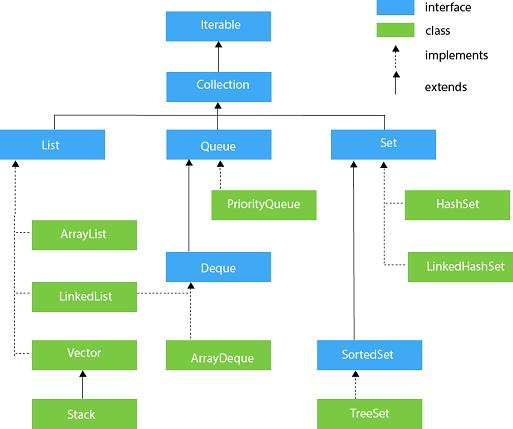
\includegraphics[width=%
0.6\textwidth]{java-collection-hierarchy}
\end{center} 

\noindent \textbf{PACCHETTI JAVA}\newline
JAVA SE $\Rightarrow$ Standard Edition \newline
JAVA EE $\Rightarrow$ Enterprise Edition \newline
JAVA ME $\Rightarrow$ Mobile Edition \newline
JAVA JDK $\Rightarrow$ linguaggio + tutte le librerie standard (java developement kit) \newline
JAVA JRE $\Rightarrow$ Solo a runtime, versione ridotta che serve solo a chi usa i programmi ma non al programmatore (java runtime enviroment) \newline
File jar  $\Rightarrow$ Archivio di tutti i pacchetti del programma \newline
JAVA JVM $\Rightarrow$ (Java virtual machine) serve per eseguire i file .jar \newline
La documentazione di java si trova on-line ed è diffusa in pacchetti che servono ad organizzare logicamente le classi, che sono organizzate in ordine alfabetico. \newline





\newpage










